\chapter{क्वांटम संख्याएँ और इलेक्ट्रॉनिक विन्यास}\label{ch:b1:quantum-numbers}

काँच की एक नली में कम दाब पर हाइड्रोजन भरिए, उसमें से विद्युत विसर्जन
गुज़ारिए और गुलाबी चमक को प्रिज़्म से देखिए। प्रकाश इंद्रधनुष की तरह नहीं
फैलता। वह चार तीखी रेखाओं में बँट जाता है --- एक लाल, एक नीली-हरी, दो
बैंगनी --- और उनके बीच कुछ नहीं। गर्म ठोस हर तरंगदैर्घ्य पर चमकता है;
हाइड्रोजन परमाणु केवल गिनी-चुनी तरंगदैर्घ्यों का उत्सर्जन करता है। इसकी
व्याख्या, जो 1913 और 1926 के बीच मिली, यह है कि परमाणु में इलेक्ट्रॉन की
ऊर्जा कोई भी मान नहीं ले सकती: वह \emph{क्वांटित} होती है। यह अध्याय इस
क्वांटमीकरण के नियम उसी रूप में देता है जिसमें रसायनज्ञ उनका उपयोग करता है
--- चार क्वांटम संख्याएँ, भरने के तीन नियम --- और उनसे हर परमाणु और आयन का
\omterm{def:b1:quantum-numbers:configuration}{इलेक्ट्रॉनिक विन्यास} निकालता है, जो अगले अध्याय की आवर्त सारणी की कुंजी है।

\begin{recall}
पुस्तक 1 (कक्षा 10) ने पहले बीस तत्वों के इलेक्ट्रॉनों को कोशों और \omterm{def:b1:quantum-numbers:orbital}{उपकोशों}
1s, 2s, 2p, 3s, 3p में रखा था, और सबसे बाहरी कोश के इलेक्ट्रॉनों को
\omterm{def:b1:quantum-numbers:configuration}{संयोजकता इलेक्ट्रॉन} कहा था। भौतिकी से हम ज्ञात मानकर यह लेते हैं कि
तरंगदैर्घ्य $\lambda$ का प्रकाश ऊर्जा
$E = h\nu = hc/\lambda$ वाले फ़ोटॉनों से बना होता है, जहाँ $h$ प्लांक स्थिरांक है
और $c$ प्रकाश की चाल।
\end{recall}

\begin{omfigure}

\includegraphics[width=0.62\linewidth]{images/book2/ai/b1-01-street-lamps.jpg}

{\small कम दाब वाले सोडियम स्ट्रीट लैंप। उनका प्रकाश लगभग एक ही नारंगी-पीली
रेखा है: हाइड्रोजन की तरह, उत्तेजित सोडियम परमाणु भी केवल कुछ निश्चित
ऊर्जाओं वाले फ़ोटॉन उत्सर्जित करता है।}
\end{omfigure}

\section{क्वांटित ऊर्जाएँ: हाइड्रोजन का स्पेक्ट्रम}

\begin{definition}[ऊर्जा स्तर, मूल अवस्था, उत्तेजित अवस्था]\label{def:b1:quantum-numbers:energy-level}
परमाणु में बंधे इलेक्ट्रॉन की ऊर्जा केवल कुछ निश्चित मान ले सकती है, जो
परमाणु के \emph{ऊर्जा स्तर}\index{ऊर्जा स्तर} कहलाते हैं। ऊर्जा का शून्य
तब लिया जाता है जब इलेक्ट्रॉन नाभिक से अनंत दूरी पर विरामावस्था में हो
(परमाणु आयनित हो), इसलिए बंधे इलेक्ट्रॉन का हर स्तर ऋणात्मक होता है। सबसे
निचला स्तर \emph{मूल अवस्था}\index{मूल अवस्था} है; बाक़ी हर स्तर एक
\emph{उत्तेजित अवस्था}\index{उत्तेजित अवस्था} है।
\end{definition}

परमाणु ऊर्जा $E_{\text{उच्च}}$ वाले स्तर से निचले स्तर
$E_{\text{निम्न}}$ पर एक फ़ोटॉन उत्सर्जित करके जाता है, और निचले से ऊँचे स्तर
पर एक फ़ोटॉन अवशोषित करके, जिसकी ऊर्जा है
\[
  h\nu = \frac{hc}{\lambda} = E_{\text{उच्च}} - E_{\text{निम्न}} .
\]
अतः रेखाओं का स्पेक्ट्रम स्तरों के बीच के अंतरों का चित्र है।

\begin{theorem}[हाइड्रोजन परमाणु के ऊर्जा स्तर]\label{thm:b1:quantum-numbers:levels}
हाइड्रोजन परमाणु के \omterm{def:b1:quantum-numbers:energy-level}{ऊर्जा स्तर} हैं
\[
  E_n = -\frac{E_R}{n^2}, \qquad n = 1, 2, 3, \dots,
  \qquad E_R = \qty{13.6}{eV},
\]
जहाँ $E_R$ रिडबर्ग ऊर्जा है (नाभिक की गति के लिए संशोधित)। \omterm{def:b1:quantum-numbers:energy-level}{मूल अवस्था}
$E_1 = \qty{-13.6}{eV}$ है और परमाणु की आयनन ऊर्जा
$E_R$ है।
% ledger: const:RyhcEV, ie:H (13.598 eV; levels computed in
% figdata/bachelor-1/hydrogen-levels.py)
\end{theorem}
\admitted

\begin{remark}[सूत्र कहाँ से आता है]\label{rem:b1:quantum-numbers:schrodinger}
यह सूत्र प्रोटॉन के क्षेत्र में इलेक्ट्रॉन का श्रोडिंगर समीकरण हल करने से
निकलता है; वह हल, और उससे मिलने वाले तरंग-फलनों की आकृतियाँ, द्वितीय वर्ष के
खंड में व्युत्पन्न की गई हैं। नील्स बोर ने यही स्तर 1913 में वृत्तीय कक्षाओं
के एक सरल मॉडल से प्राप्त किए थे, जिसे अब छोड़ दिया गया है।
\end{remark}

\begin{proposition}[रिडबर्ग सूत्र]\label{prop:b1:quantum-numbers:rydberg}
हाइड्रोजन द्वारा उत्सर्जित रेखाओं की तरंगदैर्घ्य ये हैं:
\[
  \frac{1}{\lambda} = R_H\left(\frac{1}{n_1^2} - \frac{1}{n_2^2}\right),
  \qquad n_2 > n_1 \ge 1, \qquad R_H = \frac{E_R}{hc},
\]
जो स्तर $n_2$ से नीचे स्तर $n_1$ पर संक्रमण के लिए हैं। एक ही स्तर $n_1$ पर
समाप्त होने वाली रेखाएँ एक \emph{श्रेणी} बनाती हैं: लाइमन, $n_1 = 1$ के लिए
(पराबैंगनी), बामर, $n_1 = 2$ के लिए (दृश्य), पाशन, $n_1 = 3$ के लिए
(अवरक्त)।
\end{proposition}

\begin{proof}
फ़ोटॉन परमाणु द्वारा खोई गई ऊर्जा ले जाता है:
$hc/\lambda = E_{n_2} - E_{n_1} = -E_R/n_2^2 + E_R/n_1^2
= E_R\,(1/n_1^2 - 1/n_2^2)$। $hc$ से भाग देने पर सूत्र मिलता है।
\end{proof}

\begin{example}[हाइड्रोजन की लाल रेखा]\label{ex:b1:quantum-numbers:halpha}
संक्रमण $3 \to 2$ के लिए: $\Delta E = 13.6\,(1/4 - 1/9) =
\qty{1.89}{eV}$। $hc = \qty{1240}{eV.nm}$ लेकर ($h$,
$c$ और $e$ के मानों से), $\lambda = 1240/1.89 = \qty{656}{nm}$: यही लाल रेखा है।
बामर की अन्य रेखाएँ, $4 \to 2$, $5 \to 2$, $6 \to 2$, क्रमशः 486,
434 और \qty{410}{nm} पर पड़ती हैं; अगली रेखा, $7 \to 2$, \qty{397}{nm} पर,
पहले ही पराबैंगनी में है। मापी गई तरंगदैर्घ्य, 656.3, 486.1, 434.0
और \qty{410.2}{nm}, दो हज़ार में एक भाग से भी बेहतर मेल खाती हैं; बचा हुआ
छोटा अंतर निर्वात के बजाय वायु में मापने से आता है।
% ledger: asd:Halpha, asd:Hbeta, asd:Hgamma, asd:Hdelta (computed values
% in figdata/out/bachelor-1-hydrogen-levels-balmer.dat)
\end{example}

\begin{omfigure}
\begin{tikzpicture}
\begin{axis}[
  width=0.62\linewidth, height=7.2cm,
  xmin=0, xmax=10, ymin=-14.5, ymax=0.6,
  axis x line=none, axis y line=left,
  ylabel={ऊर्जा (eV)}, ytick={-14,-12,-10,-8,-6,-4,-2,0},
  tick label style={font=\small}, label style={font=\small},
  clip=false]
\pgfplotsinvokeforeach{-13.598,-3.400,-1.511,-0.850,-0.544}{
  \draw[black!70, line width=0.7pt] (axis cs:0.3,#1) -- (axis cs:9.6,#1);}
\draw[black!40, dashed] (axis cs:0.3,0) -- (axis cs:9.6,0);
\node[font=\small, anchor=west] at (axis cs:9.7,-13.598) {$n = 1$};
\node[font=\small, anchor=west] at (axis cs:9.7,-3.400) {$n = 2$};
\node[font=\small, anchor=west] at (axis cs:9.7,-1.511) {$n = 3$};
\node[font=\small, anchor=south west] at (axis cs:9.7,0.05) {$n \to \infty$};
% Lyman
\draw[-{Stealth}, violet!70!black, thick] (axis cs:1.0,-3.400) -- (axis cs:1.0,-13.598);
\draw[-{Stealth}, violet!70!black, thick] (axis cs:1.6,-1.511) -- (axis cs:1.6,-13.598);
\draw[-{Stealth}, violet!70!black, thick] (axis cs:2.2,-0.850) -- (axis cs:2.2,-13.598);
\node[font=\small, violet!70!black, anchor=west] at (axis cs:2.4,-9) {लाइमन};
% Balmer
\draw[-{Stealth}, red!80!black, thick] (axis cs:4.4,-1.511) -- (axis cs:4.4,-3.400);
\draw[-{Stealth}, teal!80!black, thick] (axis cs:5.0,-0.850) -- (axis cs:5.0,-3.400);
\draw[-{Stealth}, blue!80!black, thick] (axis cs:5.6,-0.544) -- (axis cs:5.6,-3.400);
\node[font=\small, anchor=north] at (axis cs:5.0,-3.6) {बामर};
% Paschen
\draw[-{Stealth}, black!60, thick] (axis cs:7.8,-0.850) -- (axis cs:7.8,-1.511);
\draw[-{Stealth}, black!60, thick] (axis cs:8.4,-0.544) -- (axis cs:8.4,-1.511);
\node[font=\small, anchor=north] at (axis cs:8.1,-1.7) {पाशन};
\end{axis}
\end{tikzpicture}

{\small हाइड्रोजन के \omterm{def:b1:quantum-numbers:energy-level}{ऊर्जा स्तर}, $E_n = -\qty{13.6}{eV}/n^2$,
पैमाने के अनुसार (रिडबर्ग स्थिरांक से परिकलित); स्तर $n = 4,
5, \dots$ शून्य के ठीक नीचे सिमट जाते हैं। हर तीर एक
उत्सर्जित फ़ोटॉन है; एक ही स्तर पर समाप्त होने वाले तीर एक श्रेणी बनाते हैं।}
\end{omfigure}

\begin{omfigure}
\begin{tikzpicture}
\begin{axis}[
  width=0.9\linewidth, height=3.0cm,
  xmin=360, xmax=700, ymin=0, ymax=1,
  axis x line=bottom, axis y line=none,
  xlabel={तरंगदैर्घ्य (nm)}, xtick={400,450,500,550,600,650,700},
  tick label style={font=\small}, label style={font=\small},
  clip=false]
\fill[black!85] (axis cs:360,0) rectangle (axis cs:700,1);
% line positions: figdata/out/bachelor-1-hydrogen-levels-balmer.dat
\draw[line width=1.6pt, red!90!black] (axis cs:656.5,0) -- (axis cs:656.5,1);
\draw[line width=1.6pt, cyan!80!green] (axis cs:486.3,0) -- (axis cs:486.3,1);
\draw[line width=1.6pt, blue!70!violet] (axis cs:434.2,0) -- (axis cs:434.2,1);
\draw[line width=1.6pt, violet!75] (axis cs:410.3,0) -- (axis cs:410.3,1);
\draw[white, dashed] (axis cs:364.7,0) -- (axis cs:364.7,1);
\node[font=\small, anchor=south] at (axis cs:364.7,1.02) {सीमा};
\node[font=\small, anchor=south] at (axis cs:656.5,1.02) {$3\to2$};
\node[font=\small, anchor=south] at (axis cs:486.3,1.02) {$4\to2$};
\node[font=\small, anchor=south] at (axis cs:434.2,1.02) {$5\to2$};
\node[font=\small, anchor=south east] at (axis cs:412,1.02) {$6\to2$};
\end{axis}
\end{tikzpicture}

{\small रिडबर्ग सूत्र से परिकलित बामर रेखाएँ (निर्वात तरंगदैर्घ्य), दृश्य
पट्टी पर। आगे की रेखाएँ पराबैंगनी में \qty{364.7}{nm} पर स्थित श्रेणी-सीमा
की ओर सिमटती जाती हैं।}
\end{omfigure}

\begin{history}[बोर का परमाणु, 1913]
1913 में मैनचेस्टर में काम कर रहे 28 वर्षीय डेनिश भौतिकविद् नील्स बोर ने
प्रस्ताव रखा कि हाइड्रोजन का इलेक्ट्रॉन नाभिक के चारों ओर केवल कुछ निश्चित
कक्षाओं में घूम सकता है, और प्रकाश तब उत्सर्जित होता है जब वह एक कक्षा से
निचली कक्षा में कूदता है। उनके मॉडल ने बामर रेखाएँ ठीक-ठीक दीं, और $h$,
$e$ तथा इलेक्ट्रॉन के द्रव्यमान से रिडबर्ग स्थिरांक का मान भी। कक्षाएँ
1925--1926 की क्वांटम यांत्रिकी के आगे टिक नहीं पाईं, पर क्वांटित स्तर
टिके रहे। बोर को 1922 में भौतिकी का नोबेल पुरस्कार मिला।
\end{history}

\begin{omfigure}
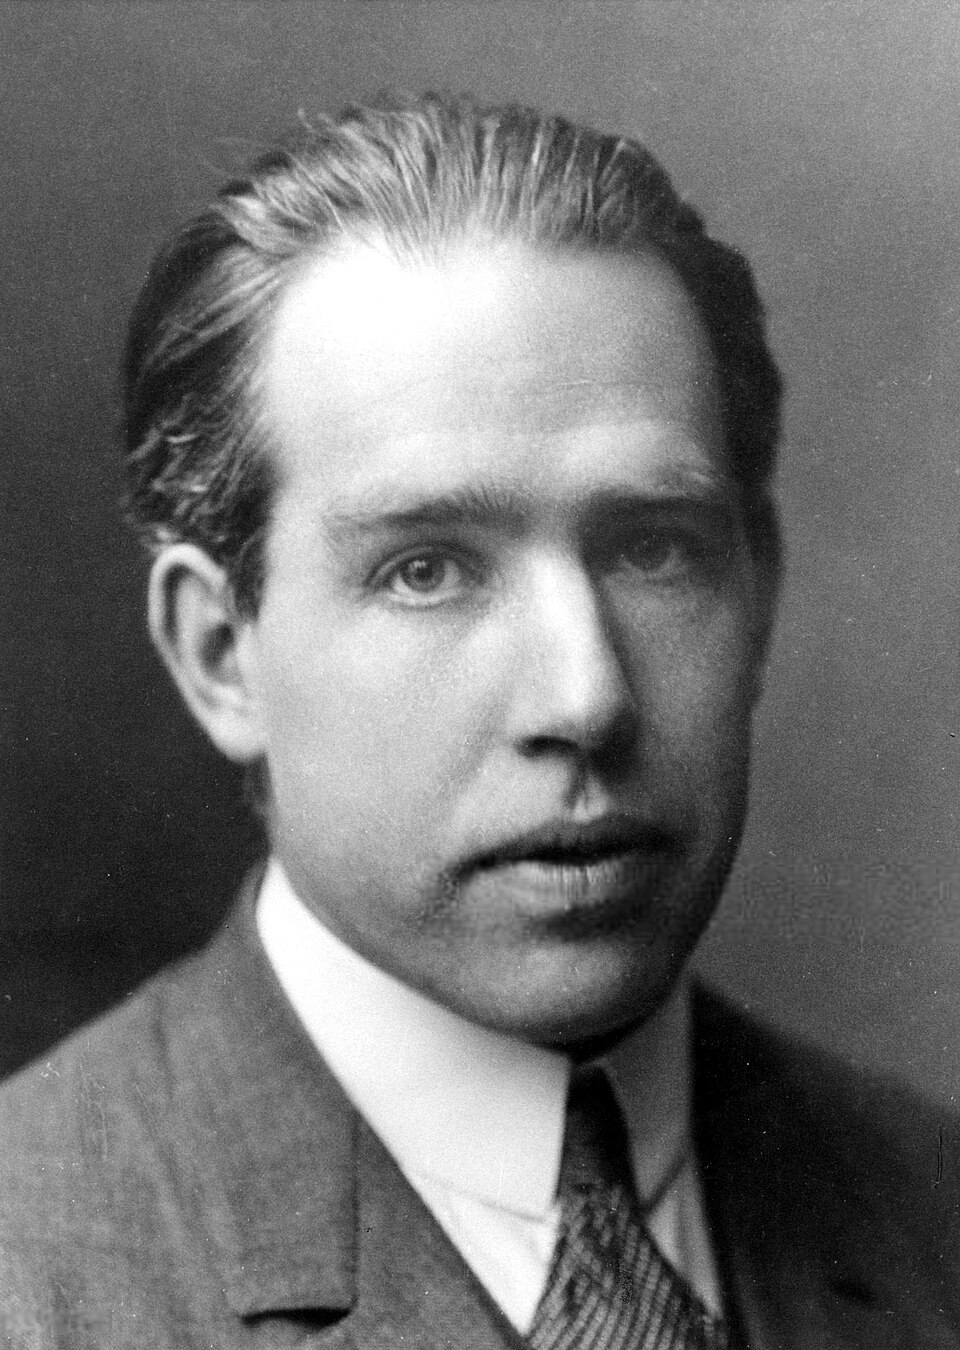
\includegraphics[width=0.26\linewidth]{images/book2/bohr.jpg}

{\small नील्स बोर (1885--1962), लगभग 1922 में।}
\end{omfigure}

\section{चार क्वांटम संख्याएँ}

अनेक इलेक्ट्रॉनों वाले परमाणु में ऊर्जाएँ अब किसी एक सूत्र से नहीं मिलतीं,
पर हर इलेक्ट्रॉन का वर्णन अब भी कुछ पूर्णांकों के एक छोटे समुच्चय से होता है:
उसकी क्वांटम संख्याएँ।

\begin{definition}[क्वांटम संख्याएँ]\label{def:b1:quantum-numbers:quantum-number}
परमाणु में किसी इलेक्ट्रॉन की अवस्था चार संख्याओं से अंकित की जाती है:
\begin{itemize}
  \item \emph{मुख्य क्वांटम संख्या}\index{मुख्य क्वांटम संख्या}
        $n = 1, 2, 3, \dots$, जो मुख्यतः ऊर्जा और आकार तय करती है;
  \item \emph{दिगंशी क्वांटम संख्या}\index{दिगंशी क्वांटम संख्या}
        (या द्वितीयक क्वांटम संख्या) $l = 0, 1, \dots, n-1$, जो आकृति
        तय करती है; $l = 0, 1, 2, 3$ को s, p, d, f लिखा जाता है;
  \item \emph{चुंबकीय क्वांटम संख्या}\index{चुंबकीय क्वांटम संख्या}
        $m_l = -l, -l+1, \dots, l$, जो अभिविन्यास तय करती है ($2l + 1$
        मान);
  \item \emph{चक्रण क्वांटम संख्या}\index{चक्रण क्वांटम संख्या}
        $m_s = +\tfrac12$ या $-\tfrac12$, इलेक्ट्रॉन का एक आंतरिक गुण, जिसे
        ऊपर या नीचे की ओर तीर से दिखाया जाता है।
\end{itemize}
\end{definition}

\begin{definition}[परमाण्वीय कक्षक, कोश, उपकोश]\label{def:b1:quantum-numbers:orbital}
\emph{परमाण्वीय कक्षक}\index{परमाण्वीय कक्षक} तीन संख्याओं $(n, l, m_l)$
से अंकित एक-इलेक्ट्रॉन अवस्था है; इसे एक खाने के रूप में बनाया जाता है,
\omorbs{}। समान $n$ वाले कक्षक एक \emph{इलेक्ट्रॉन
कोश}\index{इलेक्ट्रॉन कोश} बनाते हैं; समान $n$ और $l$ वाले कक्षक एक
\emph{उपकोश}\index{उपकोश} बनाते हैं, जिसका नाम $n$ और $l$ के अक्षर से रखा जाता है:
2p वह उपकोश है जिसमें $n = 2$, $l = 1$, और जो तीन कक्षकों
($m_l = -1, 0, 1$) से बना है।
\end{definition}

\begin{remark}[आकृतियाँ]\label{rem:b1:quantum-numbers:shapes}
s कक्षक गोलीय होता है; p कक्षक की एक अक्ष के अनुदिश दो पालियाँ होती हैं, और
तीनों 2p कक्षक $x$, $y$ और $z$ की दिशाओं में होते हैं। इन आकृतियों का
गणितीय वर्णन --- तरंग-फलन, उनके त्रिज्य और कोणीय भाग, उनके
नोड --- द्वितीय वर्ष के खंड का विषय है। इस पुस्तक में
कक्षक एक खाना है जिसमें अधिक-से-अधिक दो इलेक्ट्रॉन रह सकते हैं।
\end{remark}

\begin{proposition}[उपकोश और कोश की धारिता]\label{prop:b1:quantum-numbers:capacity}
दिगंशी संख्या $l$ वाले \omterm{def:b1:quantum-numbers:orbital}{उपकोश} में $2l + 1$ कक्षक होते हैं और उसमें
$2(2l + 1)$ इलेक्ट्रॉन आ सकते हैं: s में 2, p में 6, d में 10, f में 14। कोश $n$
में $n^2$ कक्षक होते हैं और उसमें $2n^2$ इलेक्ट्रॉन आ सकते हैं।
\end{proposition}

\begin{proof}
किसी दिए गए $l$ के लिए $m_l$ वे $2l + 1$ मान लेता है जो $-l$ से $l$ तक हैं, और
हर कक्षक में विपरीत चक्रण वाले दो इलेक्ट्रॉन रहते हैं (आगे \cref{prop:b1:quantum-numbers:pauli})।
किसी दिए गए $n$ के लिए $l$, $0$ से $n - 1$ तक जाता है, इसलिए
कक्षकों की संख्या है
\[
  \sum_{l=0}^{n-1} (2l+1) = 2\,\frac{(n-1)n}{2} + n = n^2 ,
\]
और इलेक्ट्रॉनों की संख्या $2n^2$ है: $n = 1$ से 4 के लिए 2, 8, 18, 32।
\end{proof}

\begin{example}[तीसरा कोश]\label{ex:b1:quantum-numbers:third}
$n = 3$ के लिए: $l = 0$ (3s, एक कक्षक), $l = 1$ (3p, तीन कक्षक),
$l = 2$ (3d, पाँच कक्षक, $m_l = -2, \dots, 2$): कुल नौ कक्षक और अधिकतम
18 इलेक्ट्रॉन। 3d के किसी इलेक्ट्रॉन की क्वांटम संख्याएँ, उदाहरण के लिए,
$(3, 2, -1, +\tfrac12)$ हो सकती हैं।
\end{example}

\section{विन्यास बनाना}

\begin{definition}[इलेक्ट्रॉनिक विन्यास]\label{def:b1:quantum-numbers:configuration}
किसी परमाणु या आयन का \emph{इलेक्ट्रॉनिक विन्यास}\index{इलेक्ट्रॉनिक विन्यास}
उसके भरे हुए \omterm{def:b1:quantum-numbers:orbital}{उपकोशों} की सूची है, हर \omterm{def:b1:quantum-numbers:orbital}{उपकोश} के इलेक्ट्रॉनों की संख्या घातांक के रूप में
लिखी हुई: ऑक्सीजन के लिए $1\text{s}^2 2\text{s}^2
2\text{p}^4$। सबसे बड़े $n$ वाले इलेक्ट्रॉन, अपूर्ण भरे d या f \omterm{def:b1:quantum-numbers:orbital}{उपकोश} के
इलेक्ट्रॉनों के साथ, \emph{संयोजकता
इलेक्ट्रॉन}\index{संयोजकता इलेक्ट्रॉन} हैं; शेष \emph{क्रोड
इलेक्ट्रॉन}\index{क्रोड इलेक्ट्रॉन} हैं। विन्यास को संक्षेप में लिखने के लिए
पिछली उत्कृष्ट गैस का विन्यास कोष्ठक में लिखा जाता है:
ऑक्सीजन $[\ce{He}]\,2\text{s}^2 2\text{p}^4$ है।
\end{definition}

तीन नियम \omterm{def:b1:quantum-numbers:energy-level}{मूल अवस्था} का विन्यास देते हैं।

\begin{proposition}[पाउली अपवर्जन सिद्धांत]\label{prop:b1:quantum-numbers:pauli}
एक ही परमाणु के दो इलेक्ट्रॉनों की चारों क्वांटम संख्याएँ कभी समान नहीं होतीं।
अतः एक कक्षक में अधिक-से-अधिक दो इलेक्ट्रॉन रहते हैं, और तब विपरीत
चक्रणों के साथ: \omorbs{ud}।
\end{proposition}
\admitted

\begin{proposition}[क्लेचकोव्स्की नियम]\label{prop:b1:quantum-numbers:klechkowski}
किसी उदासीन परमाणु की \omterm{def:b1:quantum-numbers:energy-level}{मूल अवस्था} में \omterm{def:b1:quantum-numbers:orbital}{उपकोश} $n + l$ के बढ़ते क्रम
में भरे जाते हैं, और समान $n + l$ होने पर $n$ के बढ़ते क्रम में:
\[
  1\text{s},\ 2\text{s},\ 2\text{p},\ 3\text{s},\ 3\text{p},\ 4\text{s},\
  3\text{d},\ 4\text{p},\ 5\text{s},\ 4\text{d},\ 5\text{p},\ 6\text{s},\
  4\text{f},\ 5\text{d},\ 6\text{p},\ 7\text{s},\ 5\text{f},\ 6\text{d},\
  7\text{p}.
\]
\end{proposition}
\admitted

\begin{remark}[एक आनुभविक नियम]\label{rem:b1:quantum-numbers:klech-empirical}
क्लेचकोव्स्की नियम (जिसे मडेलुंग नियम भी कहते हैं) प्रेक्षित विन्यासों का
सारांश है, कोई मूलभूत नियम नहीं: यह बताता है कि नाभिकीय आवेश बढ़ने के साथ
\omterm{def:b1:quantum-numbers:orbital}{उपकोश} किस क्रम में भरते हैं। अनेक इलेक्ट्रॉनों वाले परमाणु में इलेक्ट्रॉन
एक-दूसरे को प्रतिकर्षित करते हैं, इसलिए किसी \omterm{def:b1:quantum-numbers:orbital}{उपकोश} की ऊर्जा $l$ पर भी
निर्भर करती है, केवल $n$ पर नहीं: 4s इलेक्ट्रॉन, जो अपना कुछ समय नाभिक के पास बिताता
है, पोटैशियम और कैल्सियम में 3d से नीचे आ जाता है।
\end{remark}

\begin{omfigure}
\begin{tikzpicture}[font=\small, x=1.25cm, y=0.72cm]
  \foreach \n in {1,...,7} {
    \foreach \l/\s in {0/s,1/p,2/d,3/f} {
      \pgfmathtruncatemacro\ok{(\l<\n) && (\n+\l<=8)}
      \ifnum\ok=1
        \node[draw=black!50, rounded corners=2pt, minimum width=0.85cm,
          minimum height=0.5cm, fill=white] (s\n\l) at (\l,-\n) {\n\s};
      \fi
    }
  }
  \begin{scope}[on background layer]
  \foreach \la/\na/\lb/\nb in {0/1/0/1, 0/2/0/2, 1/2/0/3, 1/3/0/4, 2/3/0/5,
      2/4/0/6, 3/4/0/7, 3/5/1/7} {
    \draw[-{Stealth}, omDef, thick, opacity=0.8]
      ($(\la,-\na)+(0.5,0.42)$) -- ($(\lb,-\nb)+(-0.5,-0.42)$);
  }
  \end{scope}
  \node[anchor=west, align=left, font=\small] at (4.0,-2.5) {हर तीर का अनुसरण\\कीजिए, फिर उसके दाईं\\ओर वाले अगले तीर का};
\end{tikzpicture}

{\small क्लेचकोव्स्की आरेख। समान $n + l$ वाले \omterm{def:b1:quantum-numbers:orbital}{उपकोश} एक ही विकर्ण पर
होते हैं; विकर्णों का क्रम से अनुसरण करने पर भरने का क्रम मिलता है:
1s, 2s, 2p, 3s, 3p, 4s, 3d, 4p, 5s, \dots}
\end{omfigure}

\begin{proposition}[हुंड का नियम]\label{prop:b1:quantum-numbers:hund}
जब किसी \omterm{def:b1:quantum-numbers:orbital}{उपकोश} के इलेक्ट्रॉन समान ऊर्जा वाले कई कक्षकों में रखे जा सकते हैं,
तब \omterm{def:b1:quantum-numbers:energy-level}{मूल अवस्था} में \emph{समांतर} चक्रणों की संख्या अधिकतम होती है:
कोई भी कक्षक दोहरा भरने से पहले इलेक्ट्रॉन अलग-अलग कक्षकों में, ऊपर की ओर
चक्रण के साथ, बैठते हैं।
\end{proposition}
\admitted

\begin{definition}[अयुग्मित इलेक्ट्रॉन]\label{def:b1:quantum-numbers:unpaired}
\emph{अयुग्मित इलेक्ट्रॉन}\index{अयुग्मित इलेक्ट्रॉन} वह इलेक्ट्रॉन है जो
अपने कक्षक में अकेला हो। अयुग्मित इलेक्ट्रॉनों वाली स्पीशीज़ चुंबक की ओर
आकर्षित होती है (वह अनुचुंबकीय होती है, एक गुण जिसका अध्ययन भौतिकी में होता है)।
\end{definition}

\begin{method}[मूल अवस्था का विन्यास लिखना]\label{met:b1:quantum-numbers:configuration}
परमाणु क्रमांक $Z$ वाले परमाणु का विन्यास लिखने के लिए:
\begin{enumerate}
  \item $Z$ इलेक्ट्रॉनों को क्लेचकोव्स्की क्रम में \omterm{def:b1:quantum-numbers:orbital}{उपकोशों} में रखिए,
        अगले \omterm{def:b1:quantum-numbers:orbital}{उपकोश} से पहले हर \omterm{def:b1:quantum-numbers:orbital}{उपकोश} (2, 6, 10, 14) को भरते हुए;
  \item परिणाम को $n$ के बढ़ते क्रम में लिखिए (3d को
        $n = 3$ के साथ रखते हुए), और पिछली उत्कृष्ट गैस के क्रोड से
        संक्षेप कीजिए;
  \item अंतिम, अपूर्ण भरे \omterm{def:b1:quantum-numbers:orbital}{उपकोश} के खाने बनाइए और
        \omterm{def:b1:quantum-numbers:unpaired}{अयुग्मित इलेक्ट्रॉन} गिनने के लिए हुंड का नियम लगाइए।
\end{enumerate}
\end{method}

\begin{example}[कार्बन, नाइट्रोजन, ऑक्सीजन, आयरन]\label{ex:b1:quantum-numbers:examples}
चार परमाणुओं के लिए यह विधि देती है:
\begin{center}
\begin{tabular}{lllc}
\hline
परमाणु & विन्यास & अंतिम \omterm{def:b1:quantum-numbers:orbital}{उपकोश} & अयुग्मित \\
\hline
\ce{C} ($Z = 6$) & $[\ce{He}]\,2\text{s}^2 2\text{p}^2$ & 2p: \omorbs{u,u,} & 2 \\
\ce{N} ($Z = 7$) & $[\ce{He}]\,2\text{s}^2 2\text{p}^3$ & 2p: \omorbs{u,u,u} & 3 \\
\ce{O} ($Z = 8$) & $[\ce{He}]\,2\text{s}^2 2\text{p}^4$ & 2p: \omorbs{ud,u,u} & 2 \\
\ce{Fe} ($Z = 26$) & $[\ce{Ar}]\,3\text{d}^6 4\text{s}^2$ & 3d: \omorbs{ud,u,u,u,u} & 4 \\
\hline
\end{tabular}
\end{center}
आयरन के लिए क्लेचकोव्स्की क्रम 4s ($Z = 19, 20$) को 3d ($Z = 21$ से 30)
से पहले भरता है; पर विन्यास 3d को पहले रखकर लिखा जाता है।
% ledger: gs:Fe
\end{example}

\begin{omfigure}
\begin{tikzpicture}[font=\small]
  \begin{scope}
    \node[anchor=west] at (0,2.4) {\ce{N}: $1\text{s}^2 2\text{s}^2 2\text{p}^3$};
    \node at (0.5,1.3) {\omorbs{ud}}; \node[below] at (0.5,0.9) {1s};
    \node at (1.6,1.3) {\omorbs{ud}}; \node[below] at (1.6,0.9) {2s};
    \node at (3.1,1.3) {\omorbs{u,u,u}}; \node[below] at (3.1,0.9) {2p};
  \end{scope}
  \begin{scope}[xshift=6.2cm]
    \node[anchor=west] at (0,2.4) {\ce{Cr}: $[\ce{Ar}]\,3\text{d}^5 4\text{s}^1$};
    \node at (1.6,1.3) {\omorbs{u,u,u,u,u}}; \node[below] at (1.6,0.9) {3d};
    \node at (4.0,1.3) {\omorbs{u}}; \node[below] at (4.0,0.9) {4s};
    \node[anchor=west, text width=5.0cm] at (0,-0.1) {प्रेक्षित: छह अयुग्मित इलेक्ट्रॉन, $3\text{d}^4 4\text{s}^2$ नहीं};
  \end{scope}
\end{tikzpicture}

{\small क्वांटम खाने। हर खाना एक कक्षक है; हर तीर एक इलेक्ट्रॉन
और उसका चक्रण है। नाइट्रोजन हुंड के नियम का पालन करता है; क्रोमियम
\cref{prop:b1:quantum-numbers:exceptions} के अपवादों में से एक है।}
\end{omfigure}

\section{आयन, अपवाद और सारणी की आकृति}

\begin{proposition}[आयनों के विन्यास]\label{prop:b1:quantum-numbers:ions}
एकपरमाणुक ऋणायन का विन्यास परमाणु का विन्यास है जिसमें अतिरिक्त
इलेक्ट्रॉन क्लेचकोव्स्की क्रम के अगले स्थानों में जोड़े जाते हैं; मुख्य समूह के
तत्व का धनायन सबसे बड़े $n$ वाले इलेक्ट्रॉन खोता है। संक्रमण धातु का धनायन
अपने $n$s इलेक्ट्रॉन अपने
$(n-1)$d इलेक्ट्रॉनों से \emph{पहले} खोता है: \ce{Fe^{2+}} का विन्यास $[\ce{Ar}]\,3\text{d}^6$ है और
\ce{Fe^{3+}} का $[\ce{Ar}]\,3\text{d}^5$, न कि $[\ce{Ar}]\,3\text{d}^4
4\text{s}^2$।
% ledger: gs:Fe2+, gs:Fe3+
\end{proposition}
\admitted

\begin{remark}[भरने का क्रम हटाने का क्रम नहीं है]\label{rem:b1:quantum-numbers:order}
पोटैशियम और कैल्सियम में 4s, 3d से पहले भरता है, फिर भी संक्रमण धातुओं के
आयनों में वही पहले ख़ाली होता है। इसमें कोई विरोधाभास नहीं: \omterm{def:b1:quantum-numbers:orbital}{उपकोशों} की
ऊर्जाओं का क्रम नाभिकीय आवेश और इलेक्ट्रॉनों की संख्या के साथ बदलता है, और
संक्रमण धातु के परमाणु या आयन में 3d \omterm{def:b1:quantum-numbers:orbital}{उपकोश} 4s से नीचे होता है। क्लेचकोव्स्की
नियम केवल उदासीन परमाणुओं का वर्णन करता है।
\end{remark}

\begin{proposition}[प्रथम संक्रमण श्रेणी के दो अपवाद]\label{prop:b1:quantum-numbers:exceptions}
क्रोमियम और कॉपर के प्रेक्षित \omterm{def:b1:quantum-numbers:energy-level}{मूल अवस्था} विन्यास हैं
\[
  \ce{Cr}: [\ce{Ar}]\,3\text{d}^5 4\text{s}^1, \qquad
  \ce{Cu}: [\ce{Ar}]\,3\text{d}^{10} 4\text{s}^1 ,
\]
न कि क्लेचकोव्स्की नियम द्वारा अनुमानित $3\text{d}^4 4\text{s}^2$ और $3\text{d}^9 4\text{s}^2$:
आधा भरा या पूरा भरा d \omterm{def:b1:quantum-numbers:orbital}{उपकोश}
विशेष रूप से स्थायी होता है, और 4s तथा 3d स्तर पास-पास हैं।
% ledger: gs:Cr, gs:Cu
\end{proposition}

\begin{example}[कॉपर और उसके आयन]\label{ex:b1:quantum-numbers:copper}
\ce{Cu} का विन्यास $[\ce{Ar}]\,3\text{d}^{10} 4\text{s}^1$ है; \ce{Cu+} का
$[\ce{Ar}]\,3\text{d}^{10}$, बिना किसी \omterm{def:b1:quantum-numbers:unpaired}{अयुग्मित इलेक्ट्रॉन} के; \ce{Cu^{2+}} का
$[\ce{Ar}]\,3\text{d}^9$, एक \omterm{def:b1:quantum-numbers:unpaired}{अयुग्मित इलेक्ट्रॉन} के साथ। \ce{Zn^{2+}}, $[\ce{Ar}]\,3\text{d}^{10}$,
में कोई नहीं।
% ledger: gs:Cu+, gs:Cu2+, gs:Zn2+
\end{example}

\begin{proposition}[विन्यास और आवर्त सारणी]\label{prop:b1:quantum-numbers:table}
आवर्त सारणी का आवर्त $n$, $n$s के भरने से शुरू होता है और
$n$p के भरने पर समाप्त होता है। बीच में भरने वाले \omterm{def:b1:quantum-numbers:orbital}{उपकोश}, क्लेचकोव्स्की
नियम के अनुसार, $(n-2)$f और $(n-1)$d हैं। अतः आवर्तों में क्रमशः
$2, 8, 8, 18, 18, 32, 32$ तत्व होते हैं, और उत्कृष्ट गैसों के लिए $Z = 2, 10,
18, 36, 54, 86, 118$।
\end{proposition}

\begin{proof}
आवर्त 1 से 3 में केवल $n$s (और $n$p, जब $n \ge 2$) होते हैं: $2$, फिर
दो बार $2 + 6 = 8$। आवर्त 4 और 5 में $(n-1)$d जुड़ता है: $2 + 10 + 6 =
18$। आवर्त 6 और 7 में $(n-2)$f भी: $2 + 14 + 10 + 6 = 32$। उत्कृष्ट
गैसें हर आवर्त को बंद करती हैं: $2$, $2 + 8 = 10$, $18$, $18 + 18 = 36$,
$54$, $54 + 32 = 86$, $118$।
\end{proof}

\begin{omfigure}
\omperiodictable[colour=blocks, legend]

{\small आवर्त सारणी, भरे जा रहे अंतिम \omterm{def:b1:quantum-numbers:orbital}{उपकोश} के अनुसार रंगी हुई:
s, p, d और f ब्लॉक। हर ब्लॉक की चौड़ाई उसके \omterm{def:b1:quantum-numbers:orbital}{उपकोश} की धारिता है:
2, 6, 10 और 14।}
\end{omfigure}

\section{अभ्यास}

\begin{exercise}[$\star$]\label{exo:b1:quantum-numbers:1}
इनमें से कौन-से समुच्चय $(n, l, m_l, m_s)$ परमाणु के किसी इलेक्ट्रॉन का
वर्णन कर सकते हैं? हर अस्वीकृति का कारण बताइए।
(a) $(2, 2, 0, +\tfrac12)$; (b) $(3, 1, -1, -\tfrac12)$;
(c) $(1, 0, 0, 0)$; (d) $(4, 3, -3, +\tfrac12)$; (e) $(3, 0, 1, -\tfrac12)$।
\end{exercise}

\begin{exercise}[$\star$]\label{exo:b1:quantum-numbers:2}
\omterm{def:b1:quantum-numbers:orbital}{उपकोशों} 3d, 4f और 5p में, और कोश $n = 2$ में, कितने कक्षक हैं और
अधिक-से-अधिक कितने इलेक्ट्रॉन?
\end{exercise}

\begin{exercise}[$\star$]\label{exo:b1:quantum-numbers:3}
\ce{O}, \ce{P}, \ce{K}, \ce{Ca}
और \ce{Br} ($Z = 8, 15, 19, 20, 35$) के \omterm{def:b1:quantum-numbers:energy-level}{मूल अवस्था} विन्यास पूरे और संक्षिप्त रूप में
लिखिए, और हर एक के \omterm{def:b1:quantum-numbers:configuration}{संयोजकता इलेक्ट्रॉनों} की संख्या बताइए।
\end{exercise}

\begin{exercise}[$\star$]\label{exo:b1:quantum-numbers:4}
नाइट्रोजन, सल्फ़र और क्लोरीन के संयोजकता \omterm{def:b1:quantum-numbers:orbital}{उपकोशों} के क्वांटम खाने बनाइए, और
उनके \omterm{def:b1:quantum-numbers:unpaired}{अयुग्मित इलेक्ट्रॉन} गिनिए।
\end{exercise}

\begin{exercise}[$\star\star$]\label{exo:b1:quantum-numbers:5}
\ce{Na+}, \ce{Mg^{2+}}, \ce{Al^{3+}}, \ce{F-},
\ce{O^{2-}}, \ce{Cl-}, \ce{S^{2-}} और \ce{Ca^{2+}} के विन्यास बताइए। हर एक
किस उत्कृष्ट गैस का समइलेक्ट्रॉनी है?
\end{exercise}

\begin{exercise}[$\star\star$]\label{exo:b1:quantum-numbers:6}
\ce{Ti^{2+}}, \ce{Mn^{2+}}, \ce{Co^{2+}},
\ce{Ni^{2+}} और \ce{Zn^{2+}} ($Z = 22, 25, 27, 28, 30$) के विन्यास लिखिए और
हर एक के \omterm{def:b1:quantum-numbers:unpaired}{अयुग्मित इलेक्ट्रॉनों} की संख्या बताइए।
\end{exercise}

\begin{exercise}[$\star\star$]\label{exo:b1:quantum-numbers:7}
हाइड्रोजन के संक्रमण $4 \to 3$ में उत्सर्जित फ़ोटॉन की ऊर्जा और तरंगदैर्घ्य
परिकलित कीजिए। यह स्पेक्ट्रम के किस भाग में है?
$E_R = \qty{13.6}{eV}$ और $hc = \qty{1240}{eV.nm}$ लीजिए।
\end{exercise}

\begin{exercise}[$\star\star$]\label{exo:b1:quantum-numbers:8}
उन तत्वों को पहचानिए जिनके \omterm{def:b1:quantum-numbers:energy-level}{मूल अवस्था} विन्यास इन पर समाप्त होते हैं:
(a) $3\text{s}^2 3\text{p}^4$; (b) $4\text{s}^2 3\text{d}^{10} 4\text{p}^5$;
(c) $5\text{s}^1$; (d) $4\text{s}^2 3\text{d}^3$। (a) के अंतिम \omterm{def:b1:quantum-numbers:orbital}{उपकोश} के एक इलेक्ट्रॉन की
चारों क्वांटम संख्याएँ बताइए।
\end{exercise}

\begin{exercise}[$\star\star$]\label{exo:b1:quantum-numbers:9}
क्लेचकोव्स्की नियम की सहायता से समझाइए कि पोटैशियम का उन्नीसवाँ इलेक्ट्रॉन
3d में नहीं बल्कि 4s में क्यों जाता है, और आवर्त 3 में 18 नहीं बल्कि 8
तत्व क्यों होते हैं।
\end{exercise}

\begin{exercise}[$\star\star\star$]\label{exo:b1:quantum-numbers:10}
एक ही इलेक्ट्रॉन और आवेश $Ze$ वाले नाभिक से बने आयन के स्तर
$E_n = -Z^2 E_R/n^2$ हैं (स्वीकृत)। \ce{He+} ($Z = 2$) के लिए
आयनन ऊर्जा और संक्रमण $2 \to 1$ की तरंगदैर्घ्य परिकलित कीजिए।
हाइड्रोजन से तुलना कीजिए।
\end{exercise}

\begin{exercise}[$\star\star\star$]\label{exo:b1:quantum-numbers:11}
बताइए कि हर विन्यास \omterm{def:b1:quantum-numbers:energy-level}{मूल अवस्था} है, \omterm{def:b1:quantum-numbers:energy-level}{उत्तेजित अवस्था} है या
असंभव, और क्यों: (a) $1\text{s}^2 2\text{s}^1 2\text{p}^1$;
(b) $1\text{s}^2 2\text{s}^2 2\text{p}^7$; (c) $1\text{s}^2 2\text{p}^2$;
(d) $[\ce{Ne}]\,3\text{s}^2 3\text{p}^3$; (e) $1\text{s}^3$।
\end{exercise}

\begin{exercise}[$\star\star\star$]\label{exo:b1:quantum-numbers:12}
आयरन(III) के लवण आयरन(II) के लवणों से अधिक प्रबलता से चुंबक की ओर आकर्षित
होते हैं, और ज़िंक के लवण बिल्कुल नहीं। \ce{Fe^{2+}}, \ce{Fe^{3+}},
\ce{Mn^{2+}}, \ce{Cu^{2+}} और \ce{Zn^{2+}} को \omterm{def:b1:quantum-numbers:unpaired}{अयुग्मित
इलेक्ट्रॉनों} की संख्या के क्रम में रखिए, और यह मानकर कि आकर्षण उस संख्या के
साथ बढ़ता है, प्रेक्षण की व्याख्या कीजिए।
\end{exercise}

\section{समस्या: एक लैंप की रेखाएँ, और तीन चक्रणों वाला एक संसार}

\begin{problem}[{सप्ताहांत समस्या --- हाइड्रोजन लैंप की चार रेखाओं से
आवर्तों की लंबाई तक, और यह कि यदि इलेक्ट्रॉन की तीन चक्रण अवस्थाएँ होतीं
तो सारणी कैसी दिखती}]
\label{pb:b1:quantum-numbers:1}
पूरी समस्या में $E_R = \qty{13.6}{eV}$ और $hc = \qty{1240}{eV.nm}$ लीजिए।
दृश्य पट्टी लगभग 400 से \qty{700}{nm} तक फैली है।

\medskip
\noindent\textbf{भाग I --- हाइड्रोजन लैंप।}
\begin{enumerate}
  \item हाइड्रोजन परमाणु की ऊर्जाएँ $E_1$ से $E_4$ तक परिकलित कीजिए।
  \item संक्रमण $3 \to 2$ में उत्सर्जित फ़ोटॉन की ऊर्जा और तरंगदैर्घ्य
        परिकलित कीजिए। उसका रंग क्या है?
  \item संक्रमणों $4 \to 2$, $5 \to 2$
        और $6 \to 2$ की तरंगदैर्घ्य परिकलित कीजिए।
  \item हाइड्रोजन लैंप ठीक चार दृश्य रेखाएँ क्यों दिखाता है?
        उत्तर के समर्थन में $7 \to 2$ की तरंगदैर्घ्य परिकलित कीजिए।
  \item बामर श्रेणी की श्रेणी-सीमा परिकलित कीजिए।
  \item लाइमन की पहली रेखा, $2 \to 1$, की तरंगदैर्घ्य परिकलित कीजिए। वह
        दिखाई क्यों नहीं दे सकती?
  \item \omterm{def:b1:quantum-numbers:energy-level}{मूल अवस्था} वाले हाइड्रोजन परमाणु को आयनित कर सकने वाले फ़ोटॉन की
        अधिकतम तरंगदैर्घ्य क्या है?
\end{enumerate}

\medskip
\noindent\textbf{भाग II --- अवस्थाओं की गिनती।}
\begin{enumerate}[resume]
  \item $l$ और $m_l$ के वे मान सूचीबद्ध कीजिए जो $n = 3$ के लिए संभव हैं;
        कोश में कितने कक्षक हैं?
  \item दिखाइए कि कोश $n$ में $2n^2$ इलेक्ट्रॉन आते हैं; $n = 4$ पर लागू कीजिए।
  \item 7p तक क्लेचकोव्स्की क्रम लिखिए।
  \item सातों आवर्तों की लंबाइयाँ निकालिए।
  \item समझाइए कि 3d \omterm{def:b1:quantum-numbers:orbital}{उपकोश} आवर्त 3 में क्यों नहीं आता।
  \item उत्कृष्ट गैसों के परमाणु क्रमांक निकालिए।
\end{enumerate}

\medskip
\noindent\textbf{भाग III --- संक्रमण धातुएँ।}
\begin{enumerate}[resume]
  \item आयरन ($Z = 26$) का विन्यास लिखिए और उसके 3d
        खाने बनाइए। कितने \omterm{def:b1:quantum-numbers:unpaired}{अयुग्मित इलेक्ट्रॉन} हैं?
  \item यही प्रश्न \ce{Fe^{2+}} और \ce{Fe^{3+}} के लिए। दोनों में से किसका
        \omterm{def:b1:quantum-numbers:orbital}{उपकोश} आधा भरा है?
  \item क्रोमियम का प्रेक्षित विन्यास $[\ce{Ar}]\,3\text{d}^5
        4\text{s}^1$ है। अनुमानित विन्यास से इसकी तुलना कीजिए, और हर एक में \omterm{def:b1:quantum-numbers:unpaired}{अयुग्मित
        इलेक्ट्रॉन} गिनिए।
  \item \ce{Cu}, \ce{Cu+} और \ce{Cu^{2+}} के विन्यास बताइए।
  \item \ce{Cu+} और \ce{Cu^{2+}} में से किसमें \omterm{def:b1:quantum-numbers:unpaired}{अयुग्मित इलेक्ट्रॉन} हैं?
  \item \ce{Sc^{3+}}, \ce{Ti^{3+}}, \ce{Mn^{2+}} ($Z = 21, 22, 25$) में से
        किसमें सबसे अधिक \omterm{def:b1:quantum-numbers:unpaired}{अयुग्मित इलेक्ट्रॉन} हैं?
\end{enumerate}

\medskip
\noindent\textbf{भाग IV --- तीन चक्रणों वाला संसार।}
एक ऐसे ब्रह्मांड की कल्पना कीजिए जहाँ $n$, $l$ और $m_l$ हमारे ब्रह्मांड जैसे
ही नियमों का पालन करते हैं, क्लेचकोव्स्की क्रम नहीं बदलता, अपवर्जन सिद्धांत लागू है,
पर चक्रण संख्या $m_s$ तीन मान ले सकती है।
\begin{enumerate}[resume]
  \item एक कक्षक में कितने इलेक्ट्रॉन आ सकते हैं? संख्या $l$ वाले \omterm{def:b1:quantum-numbers:orbital}{उपकोश}
        में? कोश $n$ में?
  \item 1s, 2s, 2p, 3s और 3p की धारिताएँ बताइए।
  \item उत्कृष्ट गैस एक भरे हुए p \omterm{def:b1:quantum-numbers:orbital}{उपकोश} (पहली के लिए 1s) से आवर्त
        बंद करती है। पहली उत्कृष्ट गैस का परमाणु क्रमांक क्या है?
  \item कौन-सा परमाणु क्रमांक, पहली उत्कृष्ट गैस के बाद केवल एक इलेक्ट्रॉन के साथ,
        क्षार धातु जैसा व्यवहार करेगा?
  \item दूसरे आवर्त में कितने तत्व होंगे?
  \item इस संसार की दूसरी उत्कृष्ट गैस का परमाणु क्रमांक परिकलित कीजिए।
\end{enumerate}
\end{problem}
